\documentclass[a4paper,punct=kaiming]{ctexart}
% \documentclass[a6paper,punct=kaiming]{ctexart}

\newcommand*{\titleContent}{梁漱溟记述的顶撞毛泽东事件}
\newcommand*{\authorContent}{梁培恕}
\title{\titleContent\footnote{原载自 《炎黄春秋》 2012年第9期第53页}}
\author{\authorContent\footnote{作者为梁漱溟次子,中国社会科学院美国研究所原副编审}}
\date{}

\usepackage[hmargin=1.5in,vmargin=1in]{geometry}
% \usepackage[hmargin=.4in,vmargin=.2in]{geometry}
\usepackage{graphicx}
\usepackage[font=bf]{caption}
\usepackage[
  pdftitle={\titleContent},
  pdfauthor={\authorContent},
  hyperfootnotes=false
]{hyperref}

\setmainfont{Palatino Linotype}[
  BoldFont = PingFang SC,
  ItalicFont = KaiTi_GB2312
]

\setCJKmainfont{Songti SC}[
  BoldFont = Heiti SC,
  ItalicFont = KaiTi_GB2312
]

% \makeatletter
% \let\old@footnotetext\@footnotetext
% \renewcommand{\@footnotetext}[1]{\old@footnotetext{#1。}}
% \makeatother

\begin{document}
\maketitle

1953年7月,朝鲜停战,国家可以转向经济建设了。9月,政协全国委员会常委会扩大会议和中央人民政府委员会扩大会议召开,提出并通过了第一个五年计划——当时称为“过渡时期总路线”。会议期间,我父亲梁漱溟的发言被毛泽东批评,并引发了9月18日父亲在大会上当面顶撞毛泽东的风波。近年,我常被询及此事,并被问及父亲自己怎么看待此事以及他与毛泽东的关系。这促使我提笔,公开我所掌握的父亲一面的事实。

下面简述1953年事件的全过程。引自先父的两次发言草稿以及他自己在日记基础上整理出来的文章 《1953年9月8日至18日一段时间内的事情》 《略记9月9日至18日的一段经过》 和用作补充的文章 《我所要建议的是什么?》,都收在 《梁漱溟全集》 \footnote{山东人民出版社2005年版,以下简称 《全集》}卷七。另外还引用1953年9月至次年春夏的日记\footnote{见卷八},为使语意可解,我写了少量连缀语。此外扼要引用汪东林先生相关著作中对18日会场实况的叙述,以便将真实情况存留下来。

从我这一方面来说,我可以保证真实性。

此事的关键,是梁漱溟是否“反对过渡时期总路线”。

1953年9月8日,政协全国委员会常委会扩大会议在中南海怀仁堂召开,梁漱溟是列席者之一。当日,周恩来(当时兼任全国政协副主席)作关于过渡时期总路线的报告,征求政协委员的意见。次日,梁漱溟日记中记载:“早开小组会,予发言。午后怀仁堂开会,予请召集小组人作综合报告。周于散会时特致意希望明日发言,允之。”10日,“早九时小组会未发言”“午后怀仁堂会上发言人甚多,当告周如无时间即不发言,改用书面陈述,周答将延会一日。”11日,“无小组会。午后大会上,予发言,提三问题。周拟未能接受(李书城、章伯钧略有所言)。(后来问题发生于次日)”\footnote{以上日记,见 《全集》 卷八第502页}

现存9月11日发言稿是梁漱溟用毛笔书写的草稿。

“几天开会,〔听〕三报告,进入有计划地建国,兴奋。”“我个人曾是有这样一个梦想的人:开展一大建国运动。虽然四十年前追从旧民主革命,只知道政治改造而不知经济改造、社会改造,那是没有计划建国的。”“那时虽不晓得新民主主义,但我们要计划地建国,不走欧美旧路则千真万确。”\footnote{见 《全集》 卷七第3页}

16日发言时,已被指反对总路线,故有如下的话:“正如9月11日在政协会上我发言所说的,我实在梦想它好多好多年了。如果有人不怕费功夫,试取二、三十年来我过去的言论主张翻查一遍(现在附开一目录于此备用),那么就不难知道。”\footnote{同上,第20页}

梁漱溟两次说自己有此梦想。乡村建设运动就包括作有计划建设,但不会组织群众,发动群众,而“这原是共产党的拿手戏”\footnote{同上,第4页}。

梁漱溟的发言多有失当,可以看作过头话。如说工、青、妇都有代表他们的组织,“农会现在是什么情形呢?除了土改中起作用外,今日已不然。……群众工作谈不到,此从近几年强迫命令包办代替作风之严重即可说明。”\footnote{同上,第5页}

最后一段说及工农生活差别有如“九天九地”。“今建设重点在工业,精神所注更在此。生活之差,工人九天,农民九地。农民往城里跑,不许他跑。人才财力集中都市,虽不说遗弃吧,不说脱节吧,恐多少有点。然而农民就是人民,人民就是农民。对人民照顾不足,教育不足,安顿不好,建国如此?当初革命时农民受日本侵略者,受国民党反动派暴虐,与共产党亲切如一家人,今日已不存在此形势。”\footnote{同上,第6页}

梁漱溟在 《1953年9月8日至18日一段时间内的事情》 和 《略记9月9日至18日的一段经过》 中记载:“我说完话,农业部长李书城曾举该部如何工作,收到如何效果作答复。临末,周副主席所作总结对我已有许多答复的话,此不备记。”\footnote{同上,第16页}

事过多时,先父曾对我讲了以下情节:他归座后,看到周将秘书召来有所吩咐。作总结时依据秘书送来的材料就工农生活差别问题作了解释。这时,他第一次感到自己发言有不妥处。

他又写道:“我引用了某人所说‘工人农民生活九天九地之差’的话,嫌于破坏工农联盟而不自知。工农联盟正是我们国家政权基础,这个错误非小。当时总理似未察觉,而在他后来向主席报告我的发言之时,主席却注意了。”\footnote{同上,第11页}

其实周总理吩咐秘书送材料,表明他已注意“九天九地”的话需解释。后来拿出来批判的一直是“九天九地”,不触及亲如家人的情形“已不存在”这句话。毛泽东断定他出于恶意是这句话,而这句不能拿出来批。批即是扩散。

从梁漱溟一面去设想,批他破坏工农联盟,他会认为批得有理,与会人士同样认为批得有理。可以开一个很顺的批评会而告结束。但是偏偏选择不顺的路。

以下引自梁漱溟事后所作逐日记要\footnote{同上,第11~13页、第6页}。

12日\quad 听取彭德怀抗美援朝报告。毛主席作临时发言,“忽然说有人反对我们的总路线,替农民叫苦,大概是孔孟之徒吧! ”“中夜起来写信给主席,申明我不曾反对总路线,愿见面一为陈白。”

13日\quad “我未及剖陈”而文娱晚会开始。

15日\quad 听李富春、高岗报告,“向主席台递一字条,请求发言。主席台上宣布准许我次日发言。”

16日\quad 发言分三段。一、复述9日小组会上拥护总路线的话。二、复述11日发言,“把其中‘工人农民生活九天九地之差’不该说的话又说了出来”。“散会回家,自以为无事”。

17日\quad 发现“座席前散发一印刷件,把1949年春初我在重庆发表于 《大公报》 的两篇文章中之一篇印发出来。”“我明白是要批判我。果然,先由章伯钧起立发言,指责我许多。继由周总理在台上长篇讲话,追述往事,说我一贯反动。毛主席三次插言。”“我从座上起立,欲发言辩解,主席台上宣布会期延长一天,许我明日发言。”

18日\quad “昨天〔事态发展令人〕意外,当局认我政协发言为恶意,因为单从此〔次发言〕一事似判断不出〔恶意〕,所以追述过去之事,证明我一向反动,现在亦(依)然胸怀恶意,因此要我交待历史。”“我说:我根本没有反对总路线,而主席却诬我反对总路线。今天我要看一看毛主席有无雅量收回他的话。毛主席立刻厉声说:告诉你,我没有雅量!我正待说下去,会场内群众哄然而起……”

以上是12日至18日大概的情况。

下面是梁漱溟为18日发言准备的草稿摘句。这份草稿有一个特别,几乎不提反对总路线的事。在他看来,那几天的事很容易弄清楚,因此是着重在回答两个问题:即“一贯反动”和“想升官发财”。“周恩来居然以升官发财看我,真是妙得很!〔周称我〕‘伪君子’。”“现在空话不解决问题。……材料在手边,证人亦在此,说几个小时不难。唯一要求给我说话时间……”\footnote{同上,第7页}\textsuperscript{,}\footnote{按指当年共同组织统一建国同志会和中国民主同盟的大部分人此时也在会场,可以请他们作证}

但是周恩来当然料到他会请在座的某些人起来作证,因此事先作了准备。梁漱溟在 《略记9月9日至18日的一段经过》 中写道:“以往政府开会列席人员不多,恰值此次列席者有二百数十人之多。故颇有声势。”\footnote{同上,第18页}

以下是我对汪东林先生著 《梁漱溟问答录》 的摘录\footnote{湖南人民出版社1988年版,第137页}:

“……会场大哗,许多人大声呼喊,梁某人是胡说八道,民主权利不给反动分子,让他滚下台来,等等。”

毛泽东表现得从容缓和,说:“梁先生,你今天不要讲长了,把要点讲一讲好不好?”梁漱溟说:“刚才我说过了,希望主席给我充分的时间。”

群众不许他讲,毛泽东成了他唯一的希望,会场再次大哗。“毛泽东对会场里的人说:‘让他再讲十分钟好不好?’会场便安静下来。”

十分钟当然不够,梁再次要求给予公平待遇……

这是一个有准备的会。但是却不批评或批判梁漱溟发言破坏了工农联盟。这个题目几乎没有许多话要说。他本人和在场的党外人士就会取得一致认识,党内就更不用提了,认识一致。这样一来,似乎组织这一次斗争会目的不在此。

17日周恩来已将问题转移到过去的个人表现。18日大会的开法,体现了人民民主专政在政治生活上是怎样的。

经举手表决不让梁漱溟发言之后,大会转入批判。“发言者计有陈铭枢、史良、荣毅仁、许德珩、章伯钧、李维汉等六人。”李维汉时任统战部长,他的发言等于作总结。

据我确知,李维汉为准备开批判会,曾到李济深、张澜家中请他们二位主席(民革、民盟)发言。他们推辞了。可以想像他们不肯发言的信息传到中南海会引起什么反应——将这看作一个政治动向,促使将会议的力度加码。临时入场的二百数十人的任务是确保斗争不出纰漏,取得压倒性成果。

引人思索的是,整个事情就此戛然而止,直到1977年 《毛选》 第五卷出版才重新成为问题,至今被追问不已。

下面是戛然而止的情形。

在 《1953年9月8日至18日一段时间内的事情》 文后,梁漱溟写有附记:“此后,我即写信给政协请假在家敬候处理,对于各种集会均不去出席。……李〔维汉〕有回信,对于某些通知和请帖,说照常送给我,我出席或否,随我自己决定。关于我自请检讨一层,则嘱辛志超口头答复云不忙。……所有要给我处分的话,始终不见提,竟然一直无下文。”\footnote{见 《全集》 卷七第13页}

从日记中可以看到梁漱溟何等认真。1954年3月22日日记写道:“午后艮庸、亚、渊来谈检讨问题。艮转提兢兢业业对大局责任之义。”同年6月15日,“陈真如、林宰翁同来谈检讨问题”。次日,“发李维汉信,说学习会检讨事。”7月10日,“辛志超以李维汉语见告:检讨尚须缓些时候。”同年8月8日,“早与克木同游颐和园,星期日游人特多。在龙王庙茶座谈检讨稿甚久,克木意诚恳,亦有见地,但对我了解不够。”\footnote{以上日记,见 《全集》 卷八第523页、第533页、第535页、第538页}

文革初被红卫兵抄去的文稿、信函日记,上世纪70年代分次发还,先父检视并在其中一些文稿之后写跋语和用印。在有关1953年事件的文稿后面,他写道\footnote{见 《全集》 卷七第23页}:
\begin{quotation}\em
  1953年9月我先在政协小组会发言,后在人民政府会议席上发言,皆蓄意以旧作 《社会本位的教育系统草案》 建议于领导供参考。所谓一段心事者指此。惜我发言不慎,以致有破坏工农联盟之嫌,遭受谴责。虽当场举手表决交付政协将给我处分,而卒不见下文。盖后来领导上知我原初善意,遂从搁置也。

  \hfill 1976年“51”节核阅\hspace*{2em}

  \hfill (梁漱溟印)\hspace*{2em}
\end{quotation}

1977年4月 《毛选》 第五卷出版,改变了他的心情。4月16日看到后,曾草拟了一封致华国锋信,就当年实情有所申明。17日“恕儿来谈,不主张写信给中央领导”。18日“星贤忽来建议慎重写信,于是改写致统战部信。”同日,“以所写致统战部信遍示会上各位求指教”。晚上,“赵君迈(政协常委)来坐,美意可感。翻阅第五卷甚久,就睡。”\footnote{见 《全集》 卷八第1048页}

\begin{figure}[h]
  \centering
  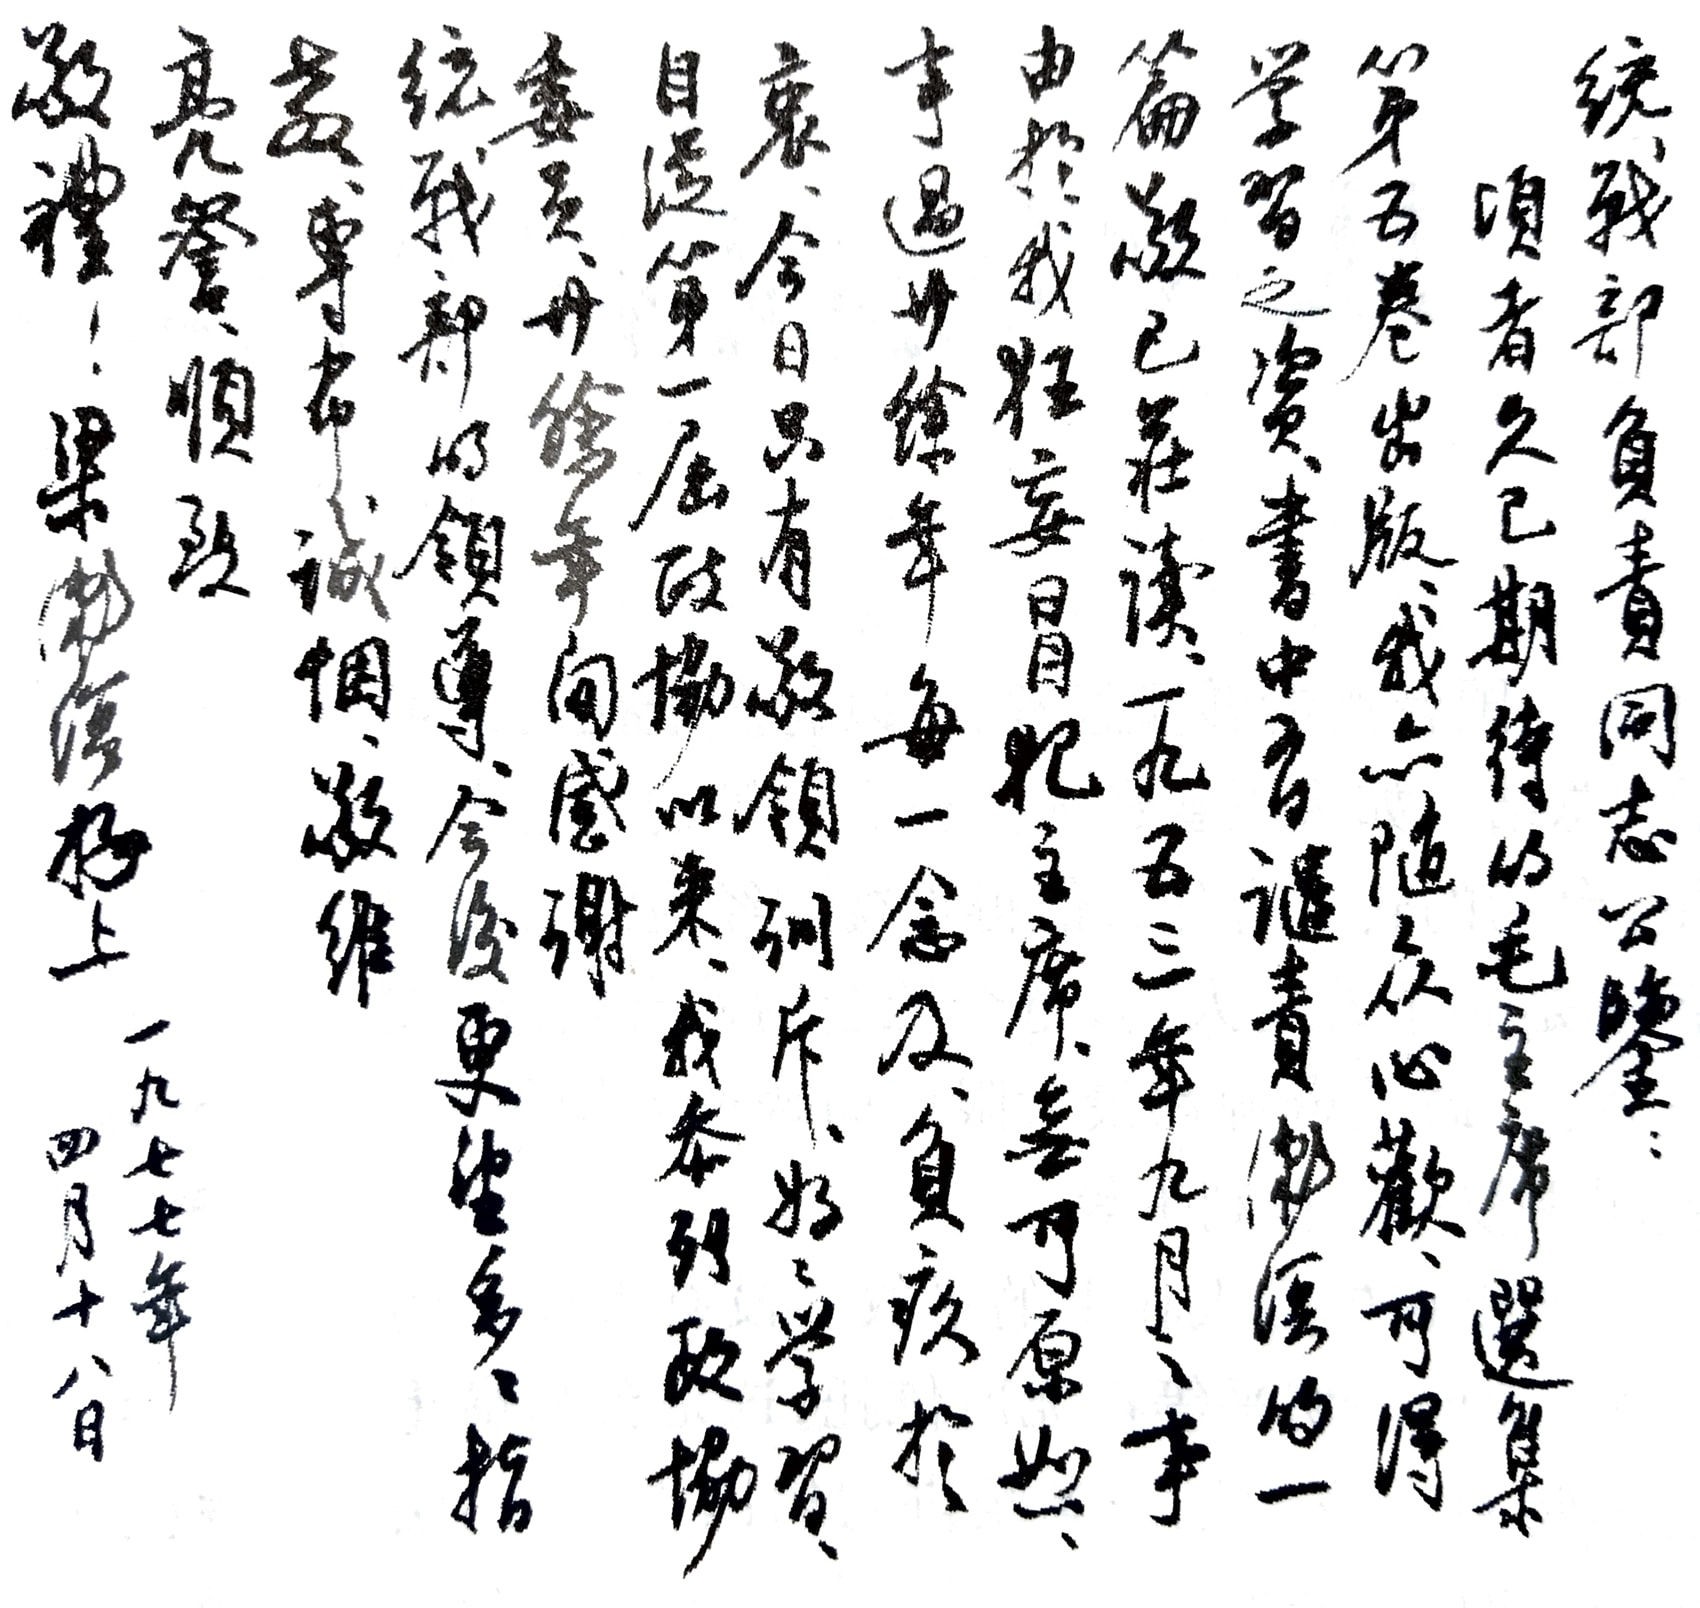
\includegraphics[width=.5\textwidth]{liang-19770418}
  \caption*{梁漱溟1977年4月18日致中共中央统战部信}
\end{figure}
\end{document}

% Local Variables:
% TeX-engine: luatex
% End:
